\documentclass[border=10pt]{standalone}

\usepackage{tikz}
\usepackage{tikzsymbols}
\usetikzlibrary{calc,patterns,shapes.geometric}

\def\centerarc[#1](#2)(#3:#4:#5){\draw[#1] ($(#2)+({#5*cos(#3)},{#5*sin(#3)})$) arc (#3:#4:#5);}

\begin{document}
	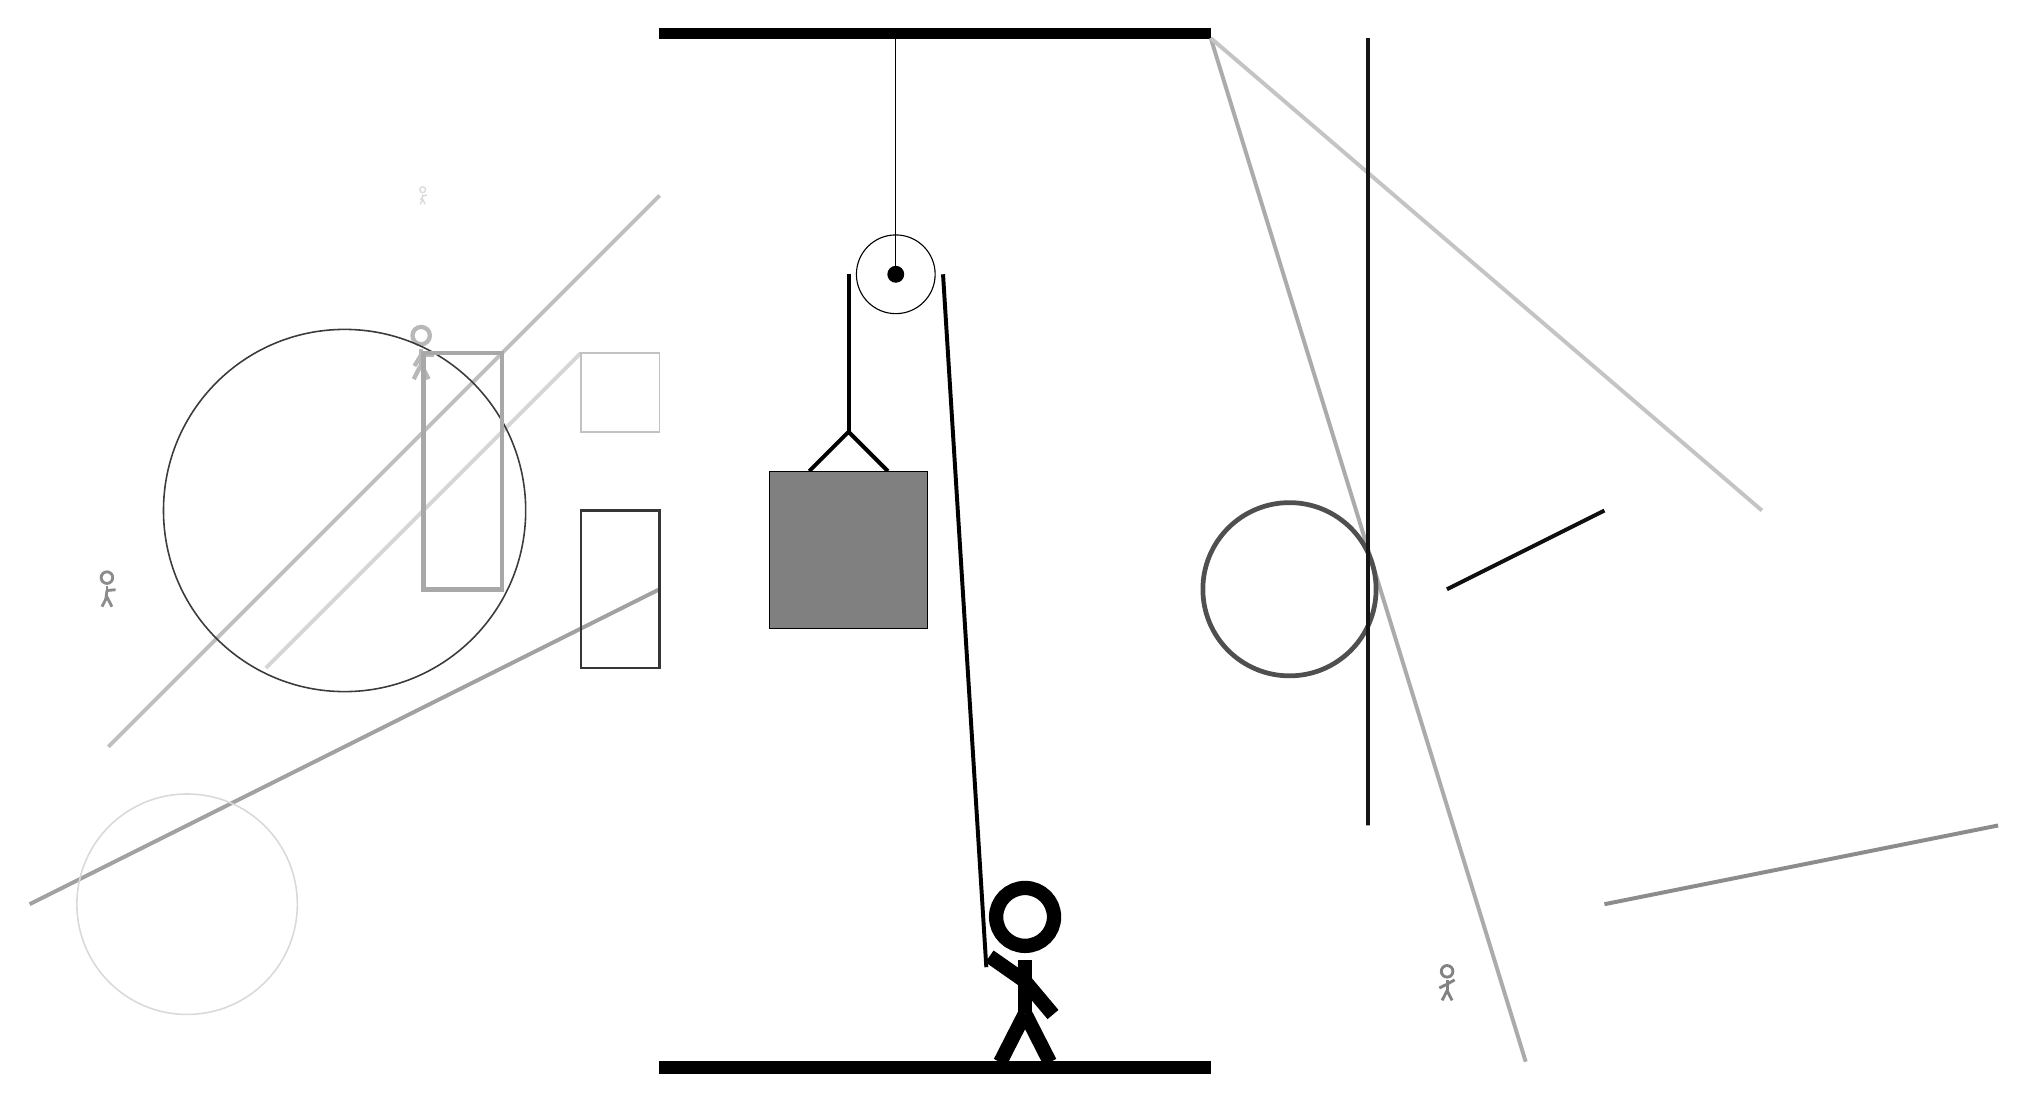
\begin{tikzpicture}
		%%%%% START %%%%%
		
		\draw[fill=black] (-2, 10) rectangle (5, 10.125);
		
		\draw (1, 7) circle (0.5);
		\draw[fill=black] (1, 7) circle (0.1);
		\draw (1, 10) -- (1, 7);
		
		\draw[line width=0.5mm, color=black!37](-2, 3) -- (-10, -1);
		
		\draw[line width=0.5mm, color=black!33](5, 10) -- (9, -3);
		\draw [line width=0.6mm, color=black!69](6, 3) circle (1.1);
		\node[line width=0.3mm, color=black!28] at (-5, 6) {\Strichmaxerl[3][59][0]};
		
		\node[line width=0.7mm, color=black!45] at (-9, 3) {\Strichmaxerl[2][83][5]};
		
		\draw[line width=0.5mm, color=black!16](-3, 6) -- (-7, 2);
		\draw[line width=0.5mm, color=black!25](-2, 8) -- (-9, 1);
		\draw[line width=0.2mm, color=black!24] (-2, 6) rectangle (-3, 5);
		\draw[line width=0.5mm, color=black!23](5, 10) -- (12, 4);
		\draw[line width=0.3mm, color=black!79] (-3, 4) rectangle (-2, 2);
		
		\node[line width=0.6mm, color=black!49] at (8, -2) {\Strichmaxerl[2][26][30]};
		\draw[line width=0.5mm, color=black!45](10, -1) -- (15, 0);
		\node[line width=0.5mm, color=black!14] at (-5, 8) {\Strichmaxerl[1][63][17]};
		
		\draw [line width=0.2mm, color=black!15](-8, -1) circle (1.4);
		\draw[line width=0.5mm, color=black!92] (7, 10) rectangle (7, 0);
		\draw [line width=0.2mm, color=black!77](-6, 4) circle (2.3);
		
		\draw[line width=0.5mm, color=black!94](10, 4) -- (8, 3);
		
		\draw[line width=0.6mm, color=black!34] (-4, 3) rectangle (-5, 6);
		
		\draw[line width=0.5mm] (-0.1, 4.5) -- (0.4, 5.0) -- (0.9, 4.5);
		\draw[fill=black!50] (-0.6, 4.5) rectangle (1.4, 2.5);
		
		\draw[line width=0.5mm] (0.4, 7) -- (0.4, 5.0);
		\centerarc[line width=0.5mm](1, 7)(0:180:0.6);
		\draw[line width=0.5mm](1.6, 7) -- (2.15, -1.8);
		
		\node at (2.6, -1.9) {\Strichmaxerl[10][-35][-50]};
		
		\draw[fill=black] (-2, -3) rectangle (5, -3.15);
		
		%%%%% END %%%%%
	\end{tikzpicture}
\end{document}